\documentclass{article}
\usepackage[utf8]{inputenc}
\usepackage{graphicx}
\usepackage{float}
\usepackage{amsmath}

\title{Machine Learning Notes: Susan Athey Course }
\author{Mason Veilleux}
\date{October 2022}

\begin{document}

\maketitle

\section{Introduction}

This paper serves as notes for each class of Susan Athey's Machine Learning and Causal Inference course. It's aim is to become a reference for future machine learning / causal inference projects that I intend to work on in the future.

\section{Class 1: Introduction}

There are two types of Machine Learning: Supervised and Unsupervised. Supervised categorizes the below:

\begin{itemize}
    \item Indepedentn Observations
    \item Stable environemtn
    \item Regression/preidciotn $E[Y | X = x]$
    \item Classification $Pr(Y=y | X = x)$
\end{itemize}

Unsupervised categorizes:

\begin{itemize}
    \item Collections of unit characterized by features
    \begin{itemize}
        \item Images
        \item Documents
        \item Individual internet activity history
    \end{itemize}
    \item Find groups of similar items
    \item Little difference across disciplines in how these methods are used
\end{itemize}

Classification: Neural nets figure out what features of image are important
Features can be used to classify images
relies on stability

Given $X_i$, is this a cat? $Pr(Y_i = CAT | X_i) = 0.95$ and $Pr(Y_i = DOG | X_i) = 0.05$

\subsection{Prediction in a Stable Environment}

Goal: Estimate $\mu (x) = E[Y | X = x]$ and minimize MSE in a new dataset where only X is observed.
\begin{itemize}
    \item MSE: $\frac{1}{I}\sum_i (Y_i - \hat{\mu} (X_i))^2$. This is the mean squared error.
    \item No matter how complex the model, the output, the prediction, is a single number.
    \item Ground truth is observed in a test set
    \item Only assumptions required: independent observations, and joint distrivution of (Y,X) same in test set as in training set
\end{itemize}

Note: minimizing MSE entails bias-variance tradeoff, and always accept some bias
\begin{itemize}
    \item Idea: if estimator too senstive to current dataset, then procedure wil be variable across datasets
    \item Models are very rich, and overfitting is a real concern. so approaches to control ovrefit is neccessary.
\end{itemize}

Idea of ML algoraiths:
\begin{itemize}
    \item Consider a family of models
    \item Use the data to select among the models or choose tuning parameters
    \item common apporach: cross-validiation
    \begin{itemize}
        \item break data into 10 folds
        \item Estimate on 9/10 of data, estimate MSE on last tenth. for each of a grid of tuning parameters
        \item Choose the parameters that minimize the MSE
    \end{itemize}
\end{itemize}

ML works well because you can accurately evaluate performance without additional assumptions
\begin{itemize}
    \item Your robotic RA then test many models to see what performs best
\end{itemize}



\subsection{Contrast with Traditional Econometrics}

Econoist have focused on the case with substantially more observations than covariates (N >> P)
\begin{itemize}
    \item In-sample MSE is a good approx. to out of sample MSE
    \item OLS is BLUE, and if overfitting is not a problem, then no need to incur bias
    \item OLS uses all the data and minimizes in-sample MSE
\end{itemize}

OLS obviously fails due to overfitting when P~N and fails entirely when P>N -- ML methods generally work when P>N.

Economists worry about estimating causal effects and identification
\begin{itemize}
    \item Causal effects
    \item Counterfactual predictions
    \item Separating correlation from causality
    \item Standard errors
    \item strucutal models incorporating behavioural assumptions
\end{itemize}

Identification probklems can not be evaulated using a hould-out set. If joint distribution observable same in training and test, then will get the sam resutsl in both

Causal methods sacrifice goodness-of-fit to focus onlt on variation in data that identifies parameters of interest.

\subsection{Key Lessons for Econometrics}

Many problems can be decomposed into preduictive and causal parts -- can use off-the-shelf ML for predictive parts

Data-driven model secltion
\begin{itemize}
    \item Tailored to econometric goals
    \begin{itemize}
        \item Focus on parameters of interest
        \item Define correct criterion for model
        \item Use data-drivedn model selection where performance can be evaluated
    \end{itemize}
    While retaining ability to do inference
\end{itemize}

ML-inspired Apporaches for Robustness

Validation
\begin{itemize}
    \item ML always has a test set
    \item Econometrics can consider alternatives
    \begin{itemize}
        \item Ruiz, Athey, and Blei (2017) evaulate on days with unusual prices
        \item Athey, Blei, Donnelly and Ruiz (2017) evaulate change in purchases before and after priec changes
        \item Tech firm applications  have many A/B tests and algorith changes
    \end{itemize}
\end{itemize}

Othre comupational approaches for structural models
\begin{itemize}
    \item Stochaistic graduet descent
    \item Variational inference (bayesian models)
\end{itemize}


See Sendhil, Mullainathan et al (JEP, AER) for key lessons about prediction in economics. See also Athey (science, 2017)

\subsection{Empirical Economics in Five Years: Athey predictions}

\begin{itemize}
    \item Regularization/data-driven model selection wil be the standard for economic models
    \item Prediction problems better appreciated
    \item Measurement using ML techniques an important subfield
    \item Textual analysis is standard
    \item Models will explicityl distinguish causal parts and predictive parts
    \item Reduced emphasis on sampling variation
    \item Model robustness emphasized on equal footing with standard errors
    \item Models with lots of latent variables
\end{itemize}



\subsection{Notes for the Mentioned Papers }
Sendhil, Mullainathan et al (JEP, AER) 
Athey (science, 2017)

\section{Class 2: Applied Machine Learning: Introduction}

The classification problem: how do we classify $Y_i$? Well, say we take a picture of a cucumber $y_i$ and actually take pictures of a lot of them $Y_i$, we then want to predict the quality of the cucumber to set a market price for each quality of cucumber (or find average price for average quality). How do we decide what a good cucumber is? Well it must be sufficiently green, have some kind of curvature that is appealing, lot's of features that us humans pick and evaluate. This is the old-style AI: deduce from human intuition, introspection.

New-style of ML: induce from training data
\begin{itemize}
    \item Take "labelled" data
    \item Fit a function $\hat{f}$ in the training sample
\end{itemize}

Each $x$ is a pixel. We also want to know how neighboring pixels relate. Lots of observations. Input layer $\rightarrow$ hidden layer (n) $\rightarrow$ output layer. Input layer is pixels, hidden layer is a function (logit model for example) output layer is a logit of logit and so on.

\subsection{Some features of ML}

\begin{itemize}
    \item Flexible, rich , data-driven models
    \item Can work with very high dimentional data
    \item Limit expressivenes to avoid overfit (regularization)
    \item Lean how much expressivenmes to allow (tuning)
    \item industry-strength tools readily available
\end{itemize}

\begin{itemize}
    \item Supervised leanring: focus on prediction
    \item Idea: turn intelleigence task into supervised-learning problem
    \item Bank decides who to give credit to
    \item Tax authority decides which returns to audit
    \item Image recognition
    \item self-driving cars
\end{itemize}

\section{Class 3: Secret Sauce of Applied Machine Learning}

Prediction problem set-up

\begin{itemize}
    \item Training data set $(y_1,x_1),.., (y_n,x_n)$ assume iid
    \begin{itemize}
        \item usually called "regression" when $y$ continuous, "classification" when $y$ is discrete
    \end{itemize}
    \item Loss function $l(\hat{y},y)$
    \item Goal:
    \item Prediction function $\hat{f}$ with low average ("risk") $L(\hat{f}) = E_{(y,x)} [l(\hat{f}(x),y)]$
    \item where $(y,x)$ distributed same as training
\end{itemize}


Language differences:
\begin{itemize}
    \item Econometrics
    \begin{itemize}
        \item y = outcome variable
        \item x = covariate
    \end{itemize}
    \item ML
    \begin{itemize}
        \item y = Label
        \item x = feature
    \end{itemize}
\end{itemize}

\subsection{How to Identify Loss/mismeasurement}

For continuous outcomes where $y \in R$ we use the squared-error loss (regression)

$L(\hat{f}) = E (\hat{f}(x) - y)^2$ or in a similar form $(l(\hat{y},y) = (\hat{y} - y)^2)$

For discrete outcome variables, we typically use ROC curves. Where we have the True positive rate on the y-axis and the false positive Rate on the x-axis. (we want the curve to be high and to the left. AUC = area under curve = higher area, more true positive rate

This can also be illustrated as a confusion matrix.



Hastie et al (2009) for approximiation-ovrefit trade-off

References: Regularization James and Stein 1961
Breiman 2001, Random Forests

\section{Approximation-Overfit Trade-Off}

THis idea is similar to the bias-variance trade-off in econometrics. Speiss distinguishes the ML approach from the Econometrics approach of this idea by splitting the data into test-train. 

Let's take a training data set that has variables $x$ and $y$ and fit a linear curve to fit that data. This curve is a decent approximation of the linear relationship between $x$ amd $y$ but let's say we want to fit a better curve, say a parabola. This approximates better. 

The trade-off reveals itself once we include the test data set. If we include the test and the training data set, we will see that we are over-fitting on the training data set. The RMSE may be low for the training data but is very high when including the test. Below is an example of this:


\begin{figure}[H]
    \centering
    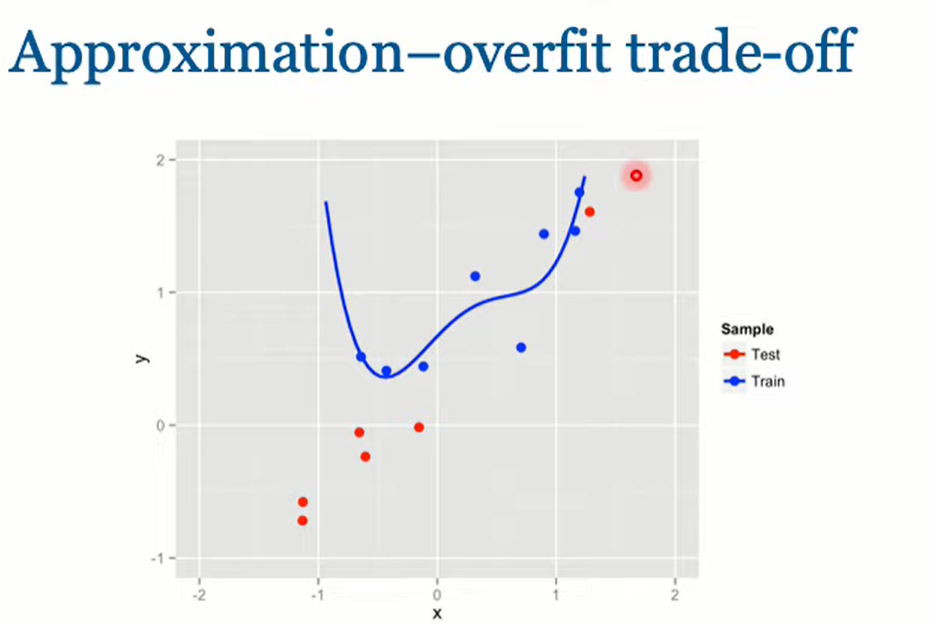
\includegraphics[scale =0.5]{approx_overfit.png}
    \caption{Caption}
    \label{fig:bias}
\end{figure}

So we can see that as we increase the degrees of freedom -- in this case the number of polynomials -- the more bias (and less variance) there is. Below is a figure that illustrates just how this works:

\begin{figure}[H]
    \centering
    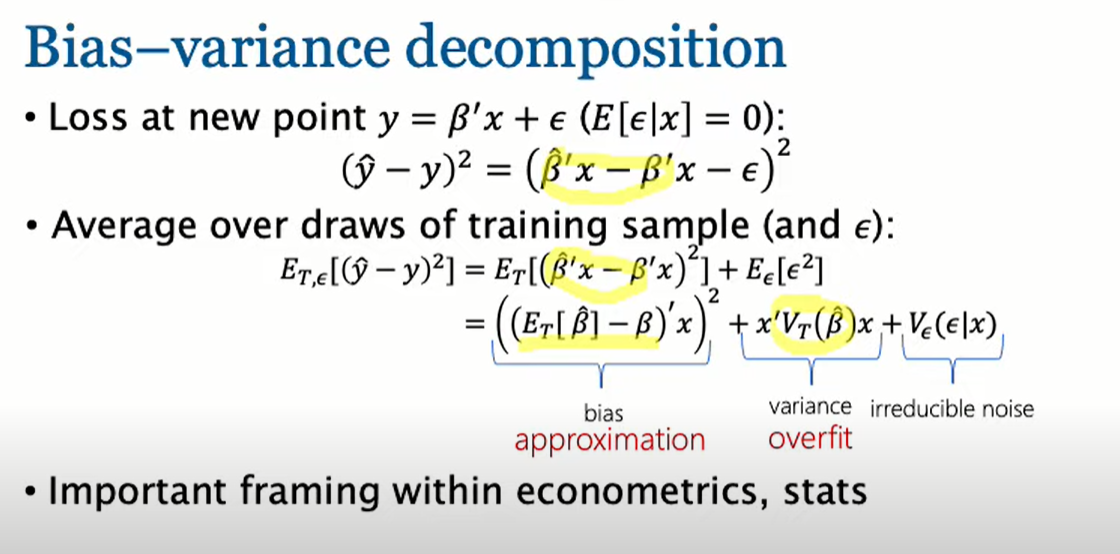
\includegraphics[scale =0.5]{bias_variance.png}
    \caption{Caption}
    \label{fig:bias_plot}
\end{figure}

Lower bias means better predictive power. What is the optimal bias/variance?

There are some key takeaways. as the model becomes more complex:

\begin{itemize}
    \item Fit True function beter (approximation)
    \item Fit noise better (overfit)
\end{itemize}

This means that we need to have flexible functional forms that express the relationship well but also need to have some tools to limit the expressiveness -- since too much expresiveness of the relationship could end up failing to explain new data. This expressiveness limiting is called regularization. 

\begin{figure}[H]
    \centering
    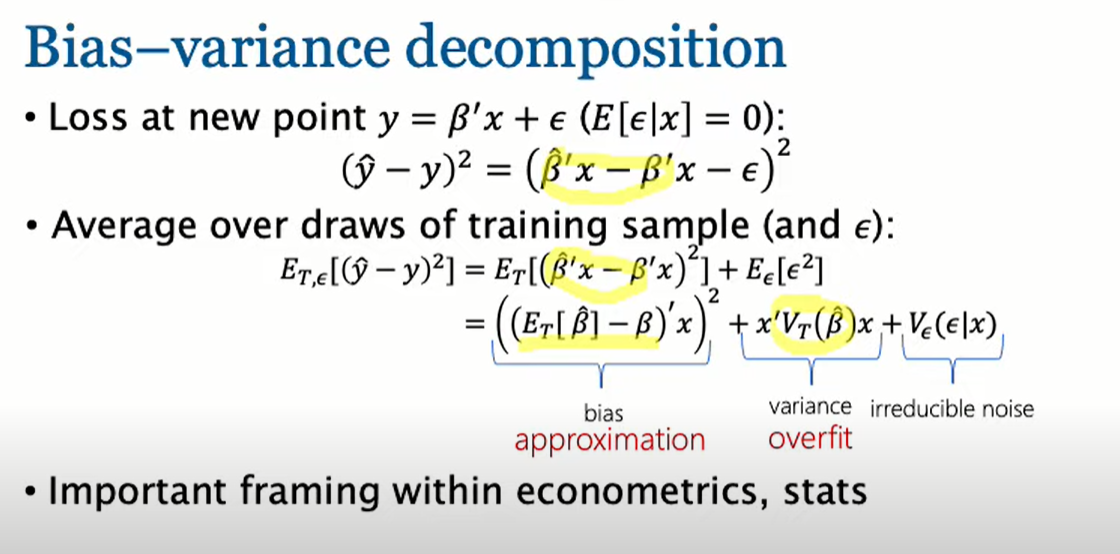
\includegraphics[scale =0.5]{bias_variance.png}
    \caption{Decomposition of Bias-Variance trade-off}
    \label{fig:overfit}
\end{figure}

\subsection{Regularization for linear regression}

When we have lots of data/variables, we can run a regresssion to predict $Y$. But as we talked about, we shouldn't use all the variables because the higher degrees of freedom of the model, the less bias but more variance we get. There are a few ways to regularize the expressiveness of the model to maximize variance and minimize bias. 

The OLS model seeks to minimize the squared residuals of the actual and predicted outcomes. 

\begin{equation}
  \phi =  min_{\hat{\beta}} \frac{1}{n} \sum_{i=1}^n (y_i - \hat{\beta}' x_i)^2
\end{equation}

if $n$ is large, like in many machine learning problems, we should regularize. This equation is called $\phi$ for short. If we regularize, the equation simply becomes:

\begin{equation}
    \phi s.t ||\hat{\beta}|| \leq c
\end{equation}

Where we not only have a minimizing condition on $\hat{\beta}$ but we also have a pseudo-norm. There are three common types of pseudo-norms that we can put on the coefficents to avoid the pitfalls of the bias-variance trade-off:

1. We can place a restriction on the number of non-zero coefficients: $||\hat{\beta}|| = \sum_{j=1}^k \hat{\beta}_j \neq 0$. In this case we can limit it to be less than or equal to $c$ variables.

2. The most common is placing a restriction on the sum of the absolute value of the estimated coefficients: $||\hat{\beta}|| = \sum_{j=1}^k |\hat{\beta}_j|$. This method is used in a LASSO regression

3. Another way of doing 2 is to do the Euclidian norm which is limiting the sume of the squared estimated coefficients:  $||\hat{\beta}||^2 = \sum_{j=1}^k \hat{\beta}^2_j$. This method is used in a Ridge regression.

Below is a figure that illustrates how these work within these regularized regression models:

\begin{figure}[H]
    \centering
    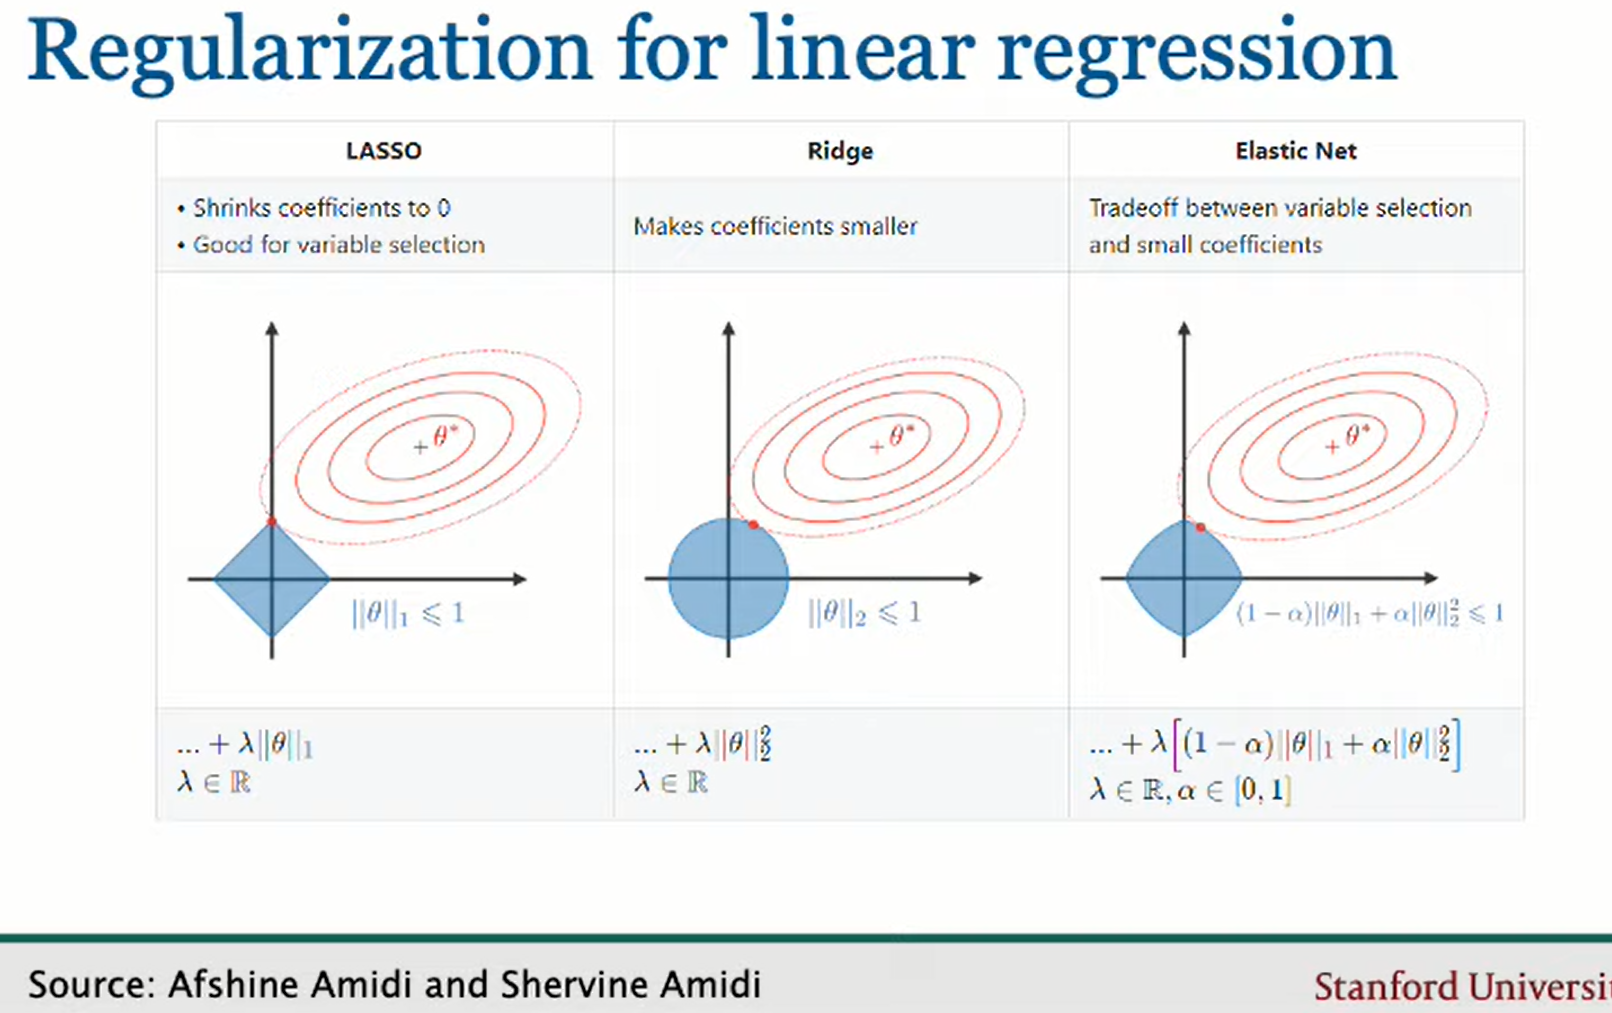
\includegraphics[scale=0.3]{reg_lin.png}
    \caption{Different Regularized Regression Models}
    \label{fig:reg_lin}
\end{figure}

where lambda $\lambda$ is a shadow cost for the number of coefficients the researcher is willing to allow. The lower the cost $\lambda$, the more coefficients. The elastic net is combindation of the Ridge and LASSO regression where $\alpha$ is the weight the researcher assumes for the LASSO-effect or the ridge-effect.

\subsection{Structure of supervised learners}

\begin{itemize}
    \item A function class
    \item A regularizer: method of limiting expressiveness
    \item An optimization Algorithm that gets us there
\end{itemize}

The issue with these linear models is that they are not very good at explaining the outcome when there are different combinations of $X$. Interactions between $X$ could be incorporated into these regularized linear regressions, but what if there are different thresholds within these interactions that produce non-linear predictions of $Y$. Well we could manually put in thresholds by binning, but then the model gets tedious. Instead, we can just use a Regression Tree which does this automatically for us. 

\subsection{Regression Tree}

The regression Tree is a different functional form than the linear models.

\begin{figure}[H]
    \centering
    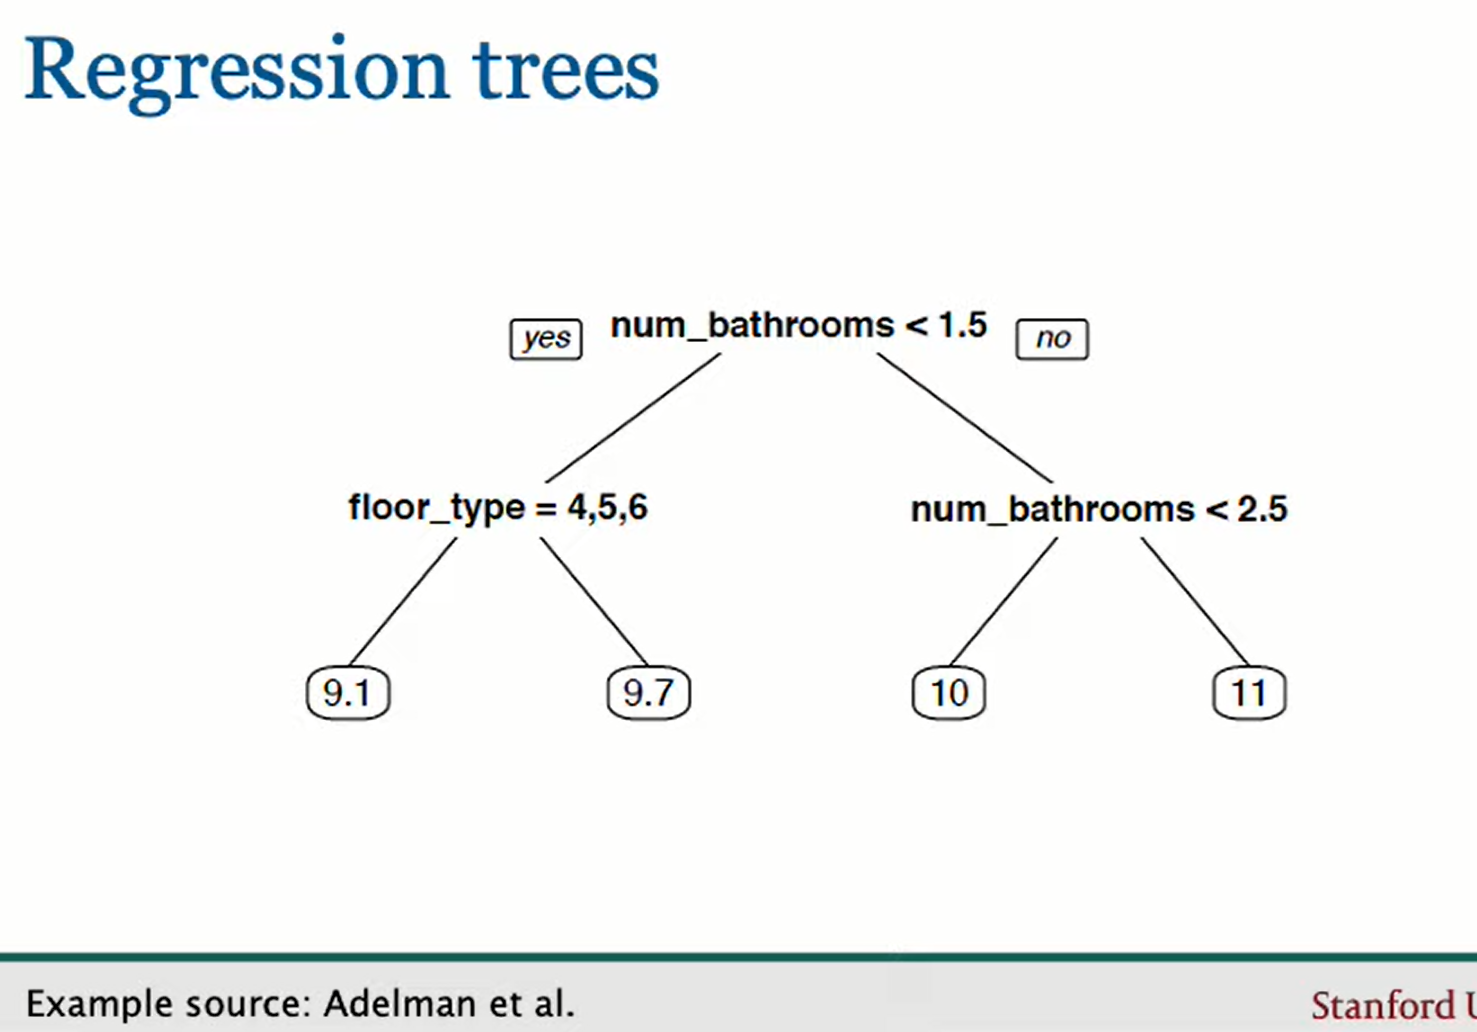
\includegraphics[scale = 0.3]{reg_tree.png}
    \caption{Regression Tree Example}
    \label{fig:my_label}
\end{figure}

Okay, cool. So just fit a regression tree and it will break your $Y$ up into bins where different interactions of $X$ are also binned. Sounds easy. But how do we find the optimal regression tree?

There are two challenges to finding the optimal tree. The first is computational. It is not easy finding an optimal tree. We solve this problem by using a greedy optimization algorithm. What this does is that it recursively finds a tree. We just pick a variable that looks best to split (maybe a discrete variable (i.e male/female , white/black, etc.). We then follow that tree down, where we pick the best variables to split till we find the optimal tree.

The second challenge is where do we stop splitting the tree? We can always improve fit by binning and more binning (adding more splits). But this means that once we test the model $\hat{f}$ on a new dataset, the predictive power is weak -- calling back to the overfit-approximation trade-off. For example, we could be predicting homes with prices and extend the tree so much that one home is in each leaf (or bin). This would not have strong predictive power. So, we need to have a way of regularizing to find the optimal number of leaves when minimizing bias and  maximizing variance. We do this through cross-validation which finds the regularization parameter.

Cross-validation is done by using 'hold-out' -- we hold out some data in our training data set to test against out-of-sample errors. We not only can hold-out some values but repeat the process and randomly hold out a group of data. A fold, $k$, in cross-validation is a dataset that has a random data group held-out. We cross-validate until all the training data has been held-out at least $n$ times. 

We can test how well our model is on our training data by taking the error term $\epsilon_i$ from each $\hat{f}_i$ trained on fold $k_i$ and produce an average of the errors $\frac{\epsilon_1 + ... + \epsilon_i}{k}$. This is called the cross-validation error. Doing this is called tuning. So we are tuning how much we need to regularize in order to find the optimal expressiveness of $\hat{f}(x)$ on $Y$. To note, we still need to test the data since the data that our model tuned on is not exact to the out-of-sample. Tuning is like a quasi-out-of-sample testing, fitting parameters as best as you can with the training dataset. Think of it as being a musician. You are trying to play (predict) Beethoven's Sonata 3 and you have taught yourself as best as you can. You then hire a tutor to tune your skills on this piece. Playing the full piece by yourself means you can play closer and closer to what is intended on the sheets (how does over-fitting work in this example -- poor finger form: optimal for one part but maybe need to adjust in the  next measure which makes the transition difficult). Visually this is illustrated as:

\begin{figure}[H]
    \centering
    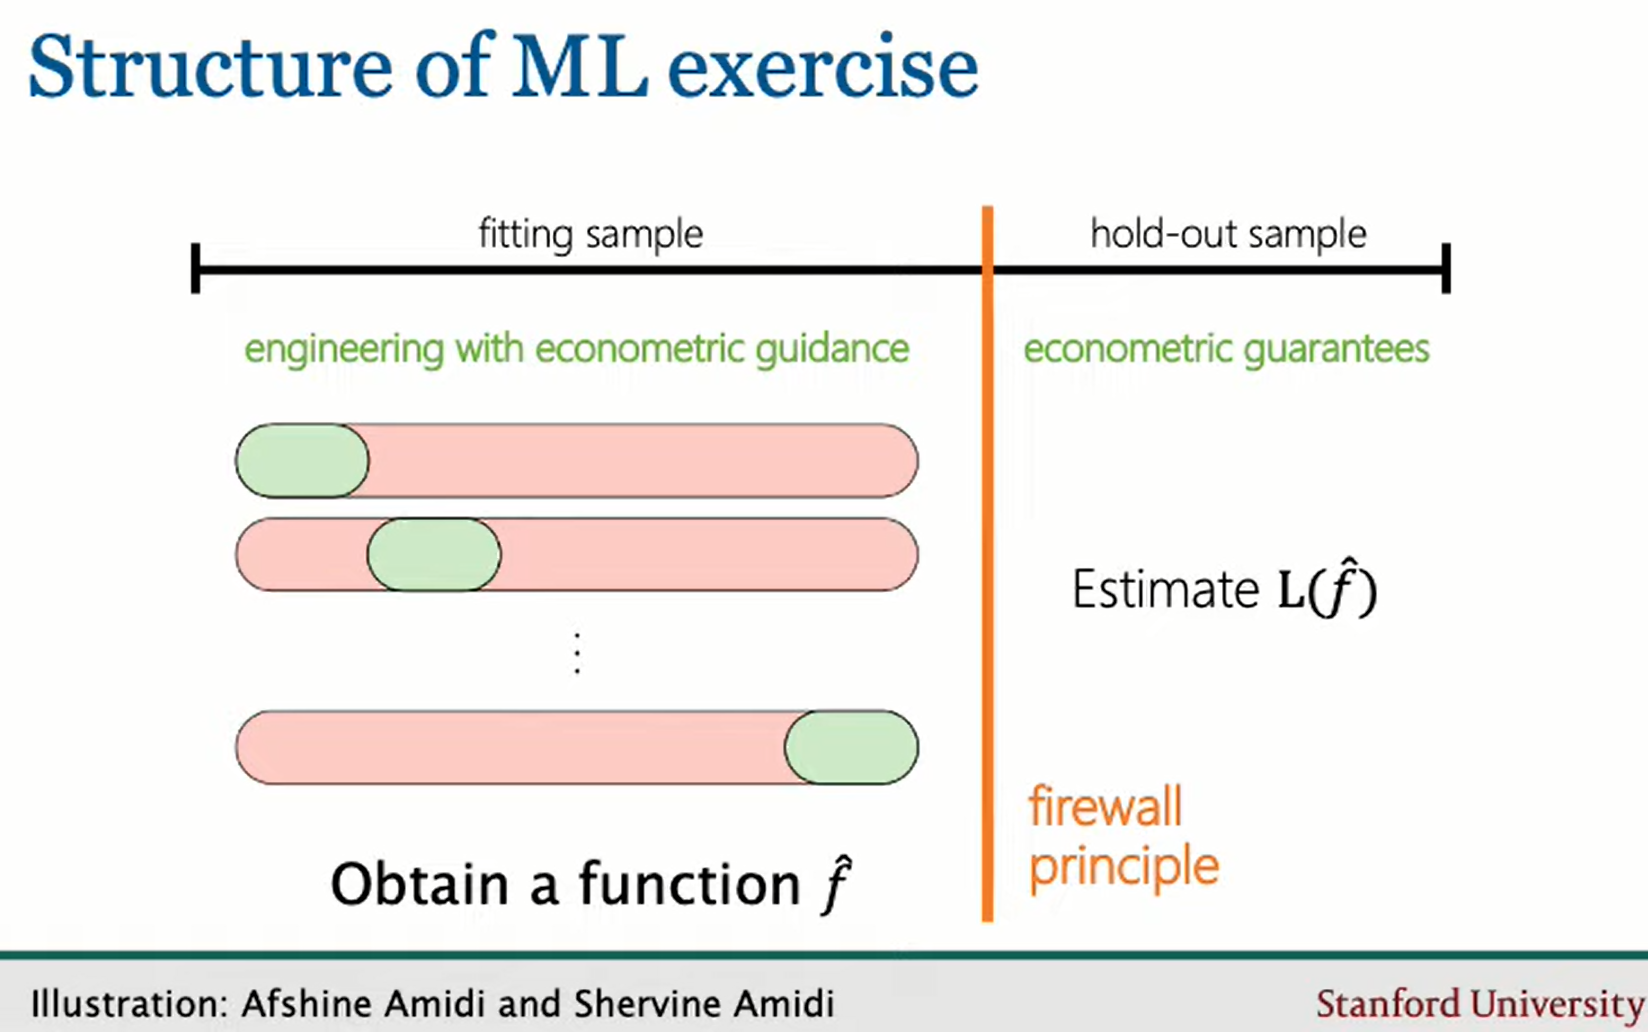
\includegraphics[scale = 0.3]{firewall.png}
    \caption{Firewall Principle}
    \label{fig:fire}
\end{figure}

This is called the firewall principle because we need to have a final hold-out sample to test our model against.

Okay, this is pretty much it. Let's recap: ML basic recap

\begin{itemize}
    \item We need flexible functional forms
    \item Limit expressiveness (regularization)
    \item Lean how much to regularize (tuning)
    \item Important researcher choices:
    \begin{itemize}
        \item Loss function: which one to optimize for?
        \item Data management / splitting
        \item Feature representation: how do we represent information in our $X$ variables
        \item Function class and regularizer
    \end{itemize}
\end{itemize}

There are lots of other different kinds of function classes and regularizers for each class:

\begin{figure}[H]
    \centering
    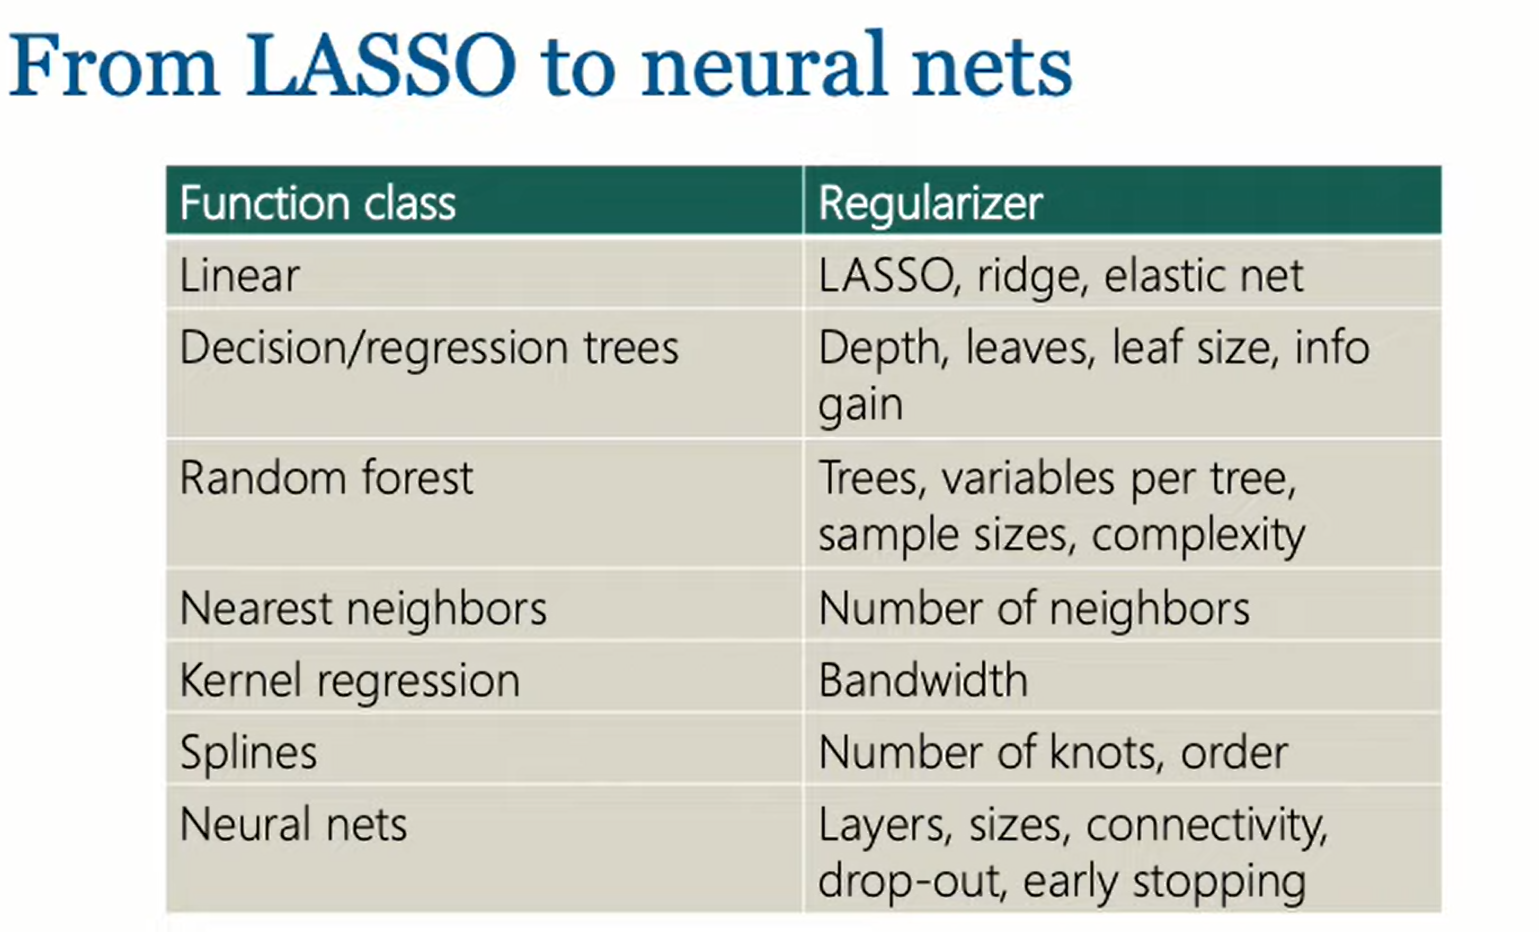
\includegraphics[scale = 0.3]{function_classes.png}
    \caption{Function Classes and their Regularizers}
    \label{fig:function_classes}
\end{figure}

Example: Neural networks can be regularized by reducing/increasing the number of layers.

Now, we can go even further. We have all these different function classes. What we can do is combine them in such a way to create a new $\hat{f}(x)$ where $\hat{f}(x) = w_1 \hat{f}_1(x) + ... +w_k \hat{f}_k(x)$. Where $w$ are the weights in each model. These combinations perform better than stand alone function classes. An example of combining multiple function classes is by combining a bunch of regression trees which is called a random forest. Where the weights are the average effects from each regression tree.


\section{Class 4 Prediction v. Estimation}

SKip -- much like previous

\section{Class 5: Introduction to Average Treatment Effects -- Part (1)}

Goal: Deploy off-the-shelf machine learning tools to support inference about average treatment effects.

Next courses will estimate treatment heterogeneity and personalization

Practice doubly robust estimation strategy (commonly used)

This course uses the potential outcomes framework. We can learn more about this framework by following Neyman 1923 and Rubin 1974. The set-up is as follows:

For a set of i.i.d subjects $i = 1,...,n$, we observe a tuple $(X_i, Y_i,W_i)$ comprised of 
\begin{itemize}
    \item A \textbf{feature vector} $X_i \in R^p$
    \item A \textbf{response} $Y_i \in R$
    \item A \textbf{treatment assignment} $W_i \in {0,1}$
\end{itemize}

In this case we assume that the treatment assignment is discrete. Will later expand on continuous (pull from Scott Cunningham Mixtape)

Following the potential outcome framework, we posit the existence of quantities $Y_i(0)$ and $Y_i(1)$ such that $Y_i = Y_i (W_i)$
\begin{itemize}
    \item Potential outcomes correspond to the response we would have measured given the i-th subject recieved treatment $(W_i =1)$ or no treatment $(W_i = 0)$
    \item the causal effect of the treatment is $Y_i(1) - Y_i(0)$
\end{itemize}

In other words, the causal effect is the difference of the potential outcomes.

The goal of this class is to estiamte the average treatment effect (ATE) which is defined as:

\begin{equation}
    \tau = E [Y_i (1) - Y_i (0)]
\end{equation}

Let's be clear, we can only observe $Y_i = Y_i (W)$. Because we cannot observe both worlds for a given $Y_i$, we need to use some tools to estimate the differences of these two worlds.

Let's take the simple example of a randomized trial.

Let's say that we are observing an outcome across units $Y_i$ given a random treatment  $W_i$ and that this random treatment is binary. Formally:

\begin{equation}
    {Y_i(0), Y_i(1)} \perp W_i
\end{equation}

Randomization is the same thing as being orthogonal (You will also see this notation used in instrumental variables).

Now we want to find our average treatment effect $\tau$. We can do this by averaging those who were treated and those who were not and then find the differences of the two groups to find a causal effect. So:

\begin{equation}
\begin{aligned}
    \tau = E[Y_i(1)] - E[Y_i(0)] \\
    = E[Y_i (1) | W_i =1 ] - E[Y_i (0) | W_i = 0] \\
    = E [Y_i | W_i = 1] - E[Y_i | W_i = 0]
    \end{aligned}
\end{equation}

Where the last line is the observable moments.

Thus, although we never observe $\tau_i = Y_i(1) - Y_i(0)$, we can consistently estimate $\tau = E[\tau_i]$ in a randomized trial.

To make things more concrete, below is a table of what we would observe in a RCT.

\begin{figure}[H]
    \centering
    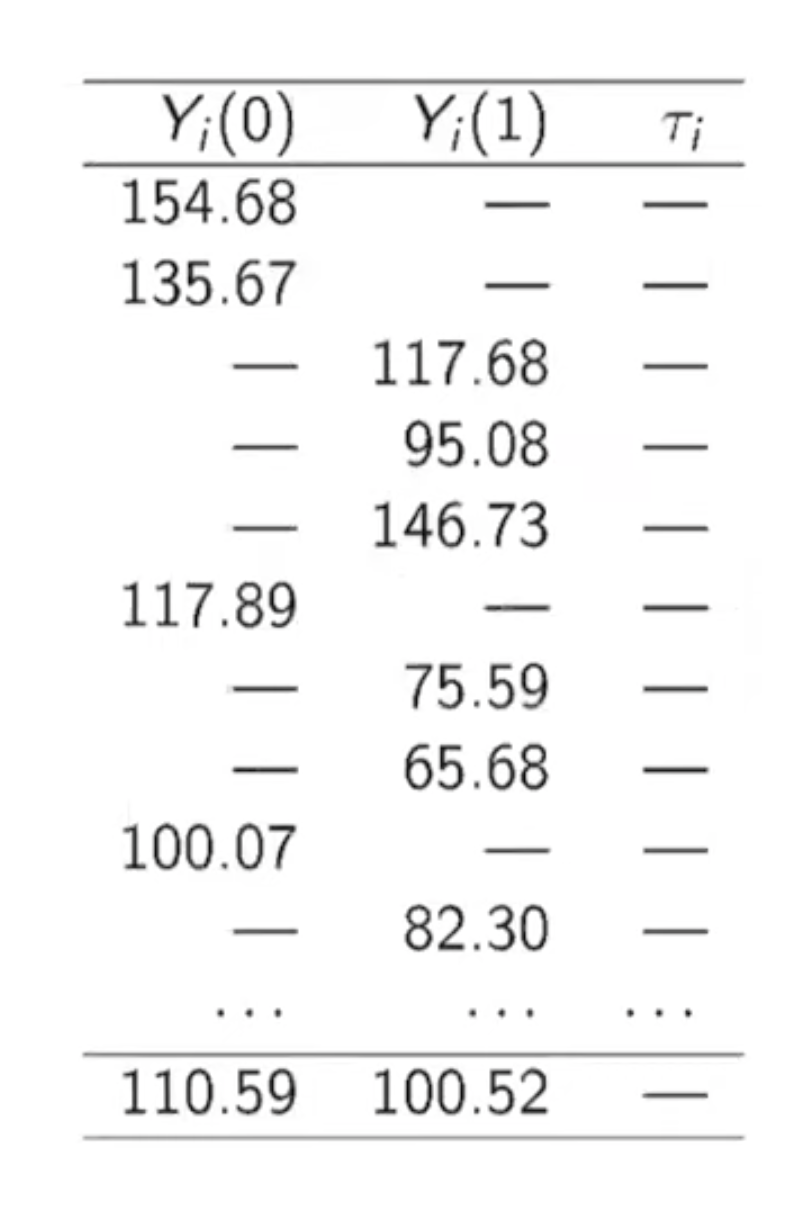
\includegraphics[scale = 0.3]{observe_RCT.png}
    \caption{Observing $Y_i$}
    \label{fig:observe_y}
\end{figure}

We would then average the columns, subtract them, and then find the causal average causal effect which would be estimated at $110.59 -100.52 = 10.07$.

Most of the time we do not have clean and clear trials that can give us a causal effect. This is because there are possible confounders that obscure the true causal effect.

Let's take an example. We want to know what the effect of obesity mitigation and prevention treatments $W_i$ on quality-adjusted life years $Y_i$. We have covariates $X_i$ that make up electronic medical records that include weight. Doctors are more likely to prescribe the treatment to patients with higher weights. With this set-up, differencing outcomes could fail to give us a valid notion of an average treatment effect.

\begin{figure}[H]
    \centering
    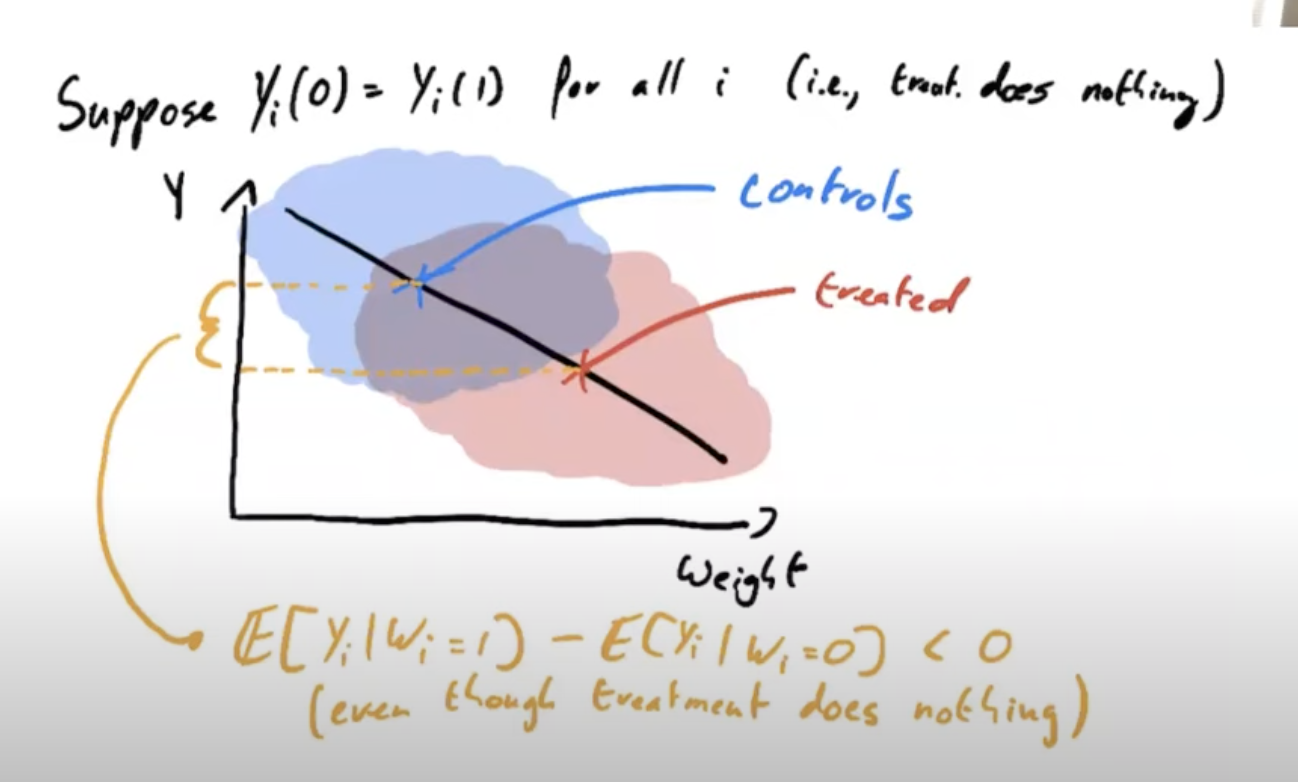
\includegraphics[scale = 0.3]{confound_rct.png}
    \caption{Confounding Problem}
    \label{fig:confound}
\end{figure}

Now, if we take the difference of the means of Y for the control group and the treated group, We'll actually get a negative estimate -- those who were treated have worse life outcomes than those who were not. So if a doctor is more likely to prescribe this treatment to someone (adult male) who is 400 pounds than to someone who is 250 pounds, the treatment could work (reduce weight) but not increase Y past those who were less likely to get the treatment. This means that weight is confounding our results due to selection bias from doctors.







\section{Class 6 Confounding in Average Treatment Effects -- Part (2)}


We want to estimate average treatment effects in a setting where treatment assignment may be associated with pre-treatment covariates X.
\begin{itemize}
    \item How can we flexibly "control" for X?

    \item Under what conditions is controlling for X enough?
\end{itemize}

\textbf{The Assumption:} Controlling for X is enough if treatment is as good as random conditionally on X

\textbf{The Questions:} What methods enable inference about the ATE given this assumption

We have the same set up before where we have an outcome determined by an orthogonal/random treatment effect. We now need to control to reduce confoundedness. This is represented as:


\begin{equation}
    [{Y_i(0), Y_i(1)} \perp W_i ] | X
\end{equation}

So this is the outcome explained by the treatment given our covariates. Controlling for this X gives the "as good as random" explanation. This assumption is commonly referred to as unconfoundedness or selection on observables (Rosenbaum \& Rubin, 1983).

(skip some of the PO notation -- repitive and intuitive)

To estimate the causal ATE using OLS we can fit the following models

\begin{equation}
    \begin{aligned}
        \hat{\beta}_{(0)} \leftarrow lm(Y_i \sim X_i subset W_i =0) \\
        \hat{\beta}_{(1)} \leftarrow lm(Y_i \sim X_i subset W_i =1) \\
    \end{aligned}
\end{equation}

We can then make prediction and obtain a treatment effect estimate as 

\begin{equation}
    \hat{\tau} = \frac{1}{n} \sum_{i=1}^n (\hat{\mu}_{(1)} (X_i) - \hat{\mu}_{(0)} (X_i)) = (\hat{\beta}_{(1)} - \hat{\beta}_{(0)} \Bar{X}
\end{equation}

where $\Bar{X} = \sum_{i=1}^n X_i$. Not that, X implicitly includes an intercept.

The pros and cons: The OLS approach hinges on having a well specified linear model. Pro: The method is simple, familiar, and well justified when the above linear model holds. Con: No guarantees if the linear model does not hold.

Machine learning allows the researcher to not assume shapes on the effects of X, W on Y. ML takes a non-parametric approach which seeks to avoid extraneous assumptions on the regression functions $\mu_{(0)}$ and $\mu_{(1)}$. The non-parametric approach still allows you to get a causal effect other than what you know to get it as $(\hat{\beta}_{(1)} - \hat{\beta}_{(0)} \Bar{X}$. So how do we go about this?

\begin{enumerate}
    \item Let's pick a ML method, and use it to predict $Y_i$ from $X_i$ and $W_i$
    \item We can then use these predictions as estimates for $\hat{\mu}_{0} (X_i)$ and $\hat{\mu}_{1} (X_i)$
    \item Estimate ATE $\hat{\tau} = \frac{1}{n} \sum_{i=1}^n (\hat{\mu}_{1} (X_i) - hat{\mu}_{0} (X_i)) $ 
\end{enumerate}
 
In many settings, machine learning methods enable accurate prediction without needing to model the shape of $\mu_{0}(x)$ and $\mu_{1}(x)$. So ML can fit either a linear or non-linear function, OLS is only linear.

(go back and do the simulation in R)

Take-aways: OLS fits linear well, not non-linear. Random forest converges ($n \rightarrow \infty$) to the consistent estimates. When linear, it converges slower than non-linear. So lots of observations solves this issue of inconsistency with ML tools. Key question is how do we make ML methods robust when we have sub-optimal finite sample performance?


\section{Class 7 Propensity Scores and Average Treatment Effects -- Part (3)}

What is a propensity score? IT is a ubiquitous concept in causal inference. Its definition is simple:

\begin{equation}
    e(x) = P [W_i = 1 | X_i = x] 
\end{equation}

i.e the propensity score measure the probability of being treated conditionally on $X_i$. In a randomized trial. the propensity score is constant $e(x) = e_0 \in (0,1)$. At least qualitatively, the variability of the propensity score gives a measure of how far we are from a randomized trial.

We can re-write the ATE in another way to incorporate the propensity score:

\begin{equation}
    \tau = E [Y_i (1) - Y_i (0)] = E [\frac{W_i Y_i}{e(X_i)} - \frac{(1-W_i) Y_i}{1 - e(X_i)}] 
\end{equation}

This implies that the following inverse-propensity weighted estimator is unbiased for the average treatment effect.

\begin{equation}
    \hat{\tau}^*_{IPW} = \frac{1}{n} \sum_{i=1}^n (\frac{W_i Y_i}{e(X_i)} - \frac{(1-W_i) Y_i}{1 - e(X_i)}) , E [\tau^*_{IPW}] = \tau
\end{equation}

IPW is inverse-propensity weighting. The same idea underlies importance weighting, Horvitz-Thomposon sampling,etc.

An issue with propensity scoring is that we do not actually know the score for each unit. We therefore need to estimate the propensity scores. How do we do that? Essentially, there is no good way to do this with ML without running into bias. 

So we went through how to get the ATE when comparing different models (Class 6). So we know that ML can give us consistent estimates for both linear and non-linear models under $n \rightarrow \infty$. Another way to find the ATE through propensity-score estimation tends to not produce consistent results (check out lecture for full explanation). However, there is another way to estimate ATE with ML: Inference via double robustness. This is the bread and butter of ML approach to estimating the ATE.

\section{Class 8 Double Robustness and Average Treatment Effects -- Part (4)}

This is the method you want to use to estimate ATE with machine learning.

So the issue that we run into when using ML to estiamte ATE is that we need lots of data for our $\hat{\tau}$ to converge to $\tau$. But when we have sufficiently large data, our $\hat{f}$ from an out of the box ML approach is consistent for both linear and non-linear data. As far as we know, the ability to converge on $\tau$ is a predictive black box: A machine learning method that can provide "pretty good" estimates of regression functions that satisfy:

\begin{equation}
    \sqrt{E[ (\hat{\mu}_{(w)}(X_i) - \mu_{(w)}(X_i))^2  ]} << \frac{1}{^4\sqrt{n}}
\end{equation}

which this is the conditional response function.

\begin{equation}
    \sqrt{E[ (\hat{e}(X_i) - e_{(w)}(X_i))^2  ]} << \frac{1}{^4\sqrt{n}}
\end{equation}


and this is the propensity score. The estimates converge according to $\frac{1}{^4\sqrt{n}}$. There is research that explains why we use $\frac{1}{^4\sqrt{n}}$ -- essentially, assuming a 4-th root rate is a way of saying the machine learning method is pretty accurate, but does not achieve parametric rates. We tune for Root Mean Squared Error (RMSE) since this is what we are converging too (right?).

Okay, here's the juice. The estimator we want to use will combine both the conditional response function (outcome regression) and the propensity score and compare the errors to find the optimal prediction. This estimator is called \textbf{Augmented Inverse- Propensity Weighting} or AIPW. Below is the functional form:

\begin{equation}
    \hat{\tau} = \frac{1}{n} \ sum_{i=1}^n (\hat{\mu}_{(1)} (X_i) - \hat{\mu}_{(0)} (X_i) + \frac{W_i}{\hat{e}(X_i)} (Y_i - \hat{\mu}(1) (X_i)) - \frac{1- W_i}{1- \hat{e}(X_i)}(Y_i - \hat{\mu}_{(0)}(X_i)) )
\end{equation}

This feels complicated. Let's break it down into two parts:

\begin{equation}
    \hat{\tau}_{AIPW} = D + R
\end{equation}

\begin{equation}
    D = \frac{1}{n} \ sum_{i=1}^n (\hat{\mu}_{(1)} (X_i) - \hat{\mu}_{(0)} (X_i))
\end{equation}

$D$ is the direct regression adjustment estimator using $\hat{\mu}_{(w)} (x)$


\begin{equation}
    R = \frac{1}{n} \ sum_{i=1}^n (\frac{W_i}{\hat{e}(X_i)} (Y_i - \hat{\mu}(1) (X_i)) - \frac{1- W_i}{1- \hat{e}(X_i)}(Y_i - \hat{\mu}_{(0)}(X_i)) )
\end{equation}

$R$ is an Inverse-Propensity Weight estimator applied to the residuals $Y_i - \hat{\mu}_{(W_i)} (X_i)$.

Qualitatively, AIPW uses propensity weighting on the residual to debias the direct estimate. The residuals in this case are represented in $R$ as $Y_i - \hat{\mu}_{(0)}(X_i)$ for the firs term in $R$. So we first estimate using the regression function, then adjust with IPW.

Implementing this in R is easy using the grf package. 

  \begin{verbatim}
    # AIPW in R
    attach(grf)
    cf = causal_forest(X,Y,W)
    ate.hat = average_treatment_effect(cf)
    \end{verbatim}

The first function does the AIPW, estimating the regression and then appling IPW on the residuals. The second function extracts the results to form doubly robust scores.

We are first going to touch on inference with AIPW and then go into some details.

\subsection{Inference with AIPW}

So when we get our $\hat{\tau}$, we can take that value as the average, but we need to get the confidence intervals. We can do this by the following (just taking screen shot -- too much writing)

\begin{figure}[H]
    \centering
    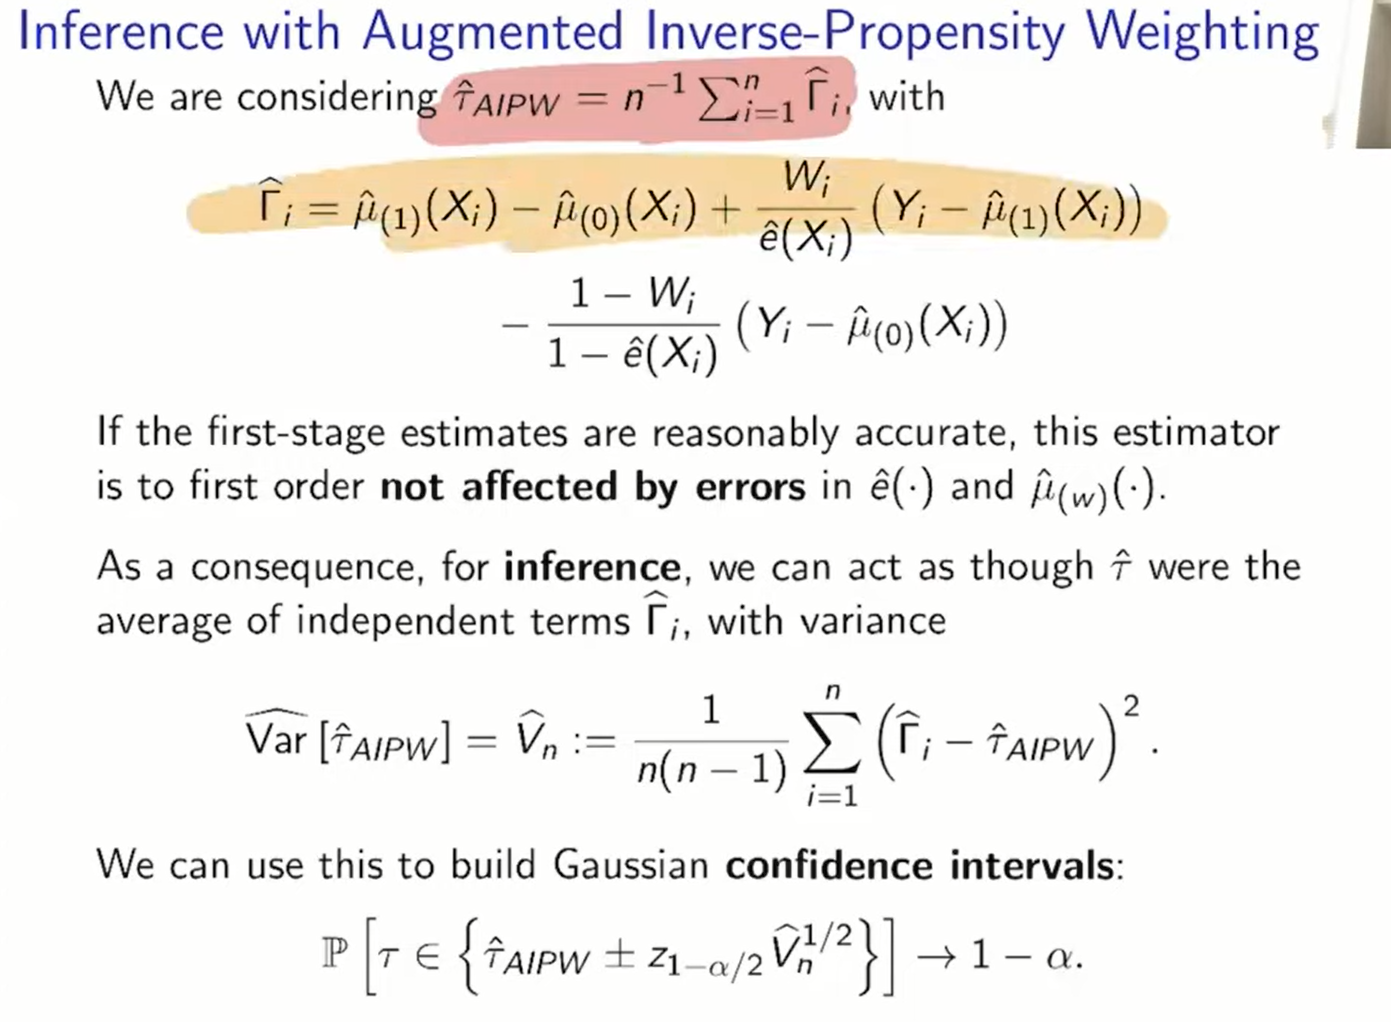
\includegraphics[scale = 0.3]{inference_aipw.png}
    \caption{Inference for AIPW}
    \label{fig:inference_aipw}
\end{figure}

\subsection{Detail 1: Cross-Fitting}

This is the same idea as cross-validation. So we cut into folds and do leave-one-out estimation. See Chernozhukov et al (2018) for AIPW flexible efficiency


\begin{figure}[H]
    \centering
    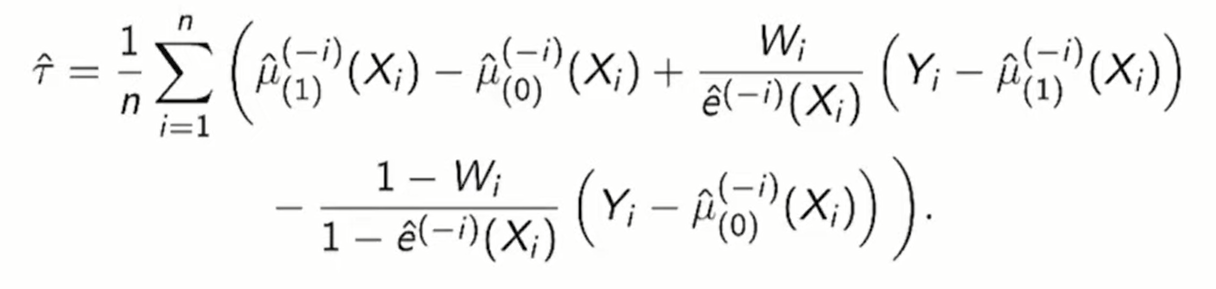
\includegraphics[scale = 0.3]{cross_fitting.png}
    \caption{Cross-Fitting for AIPW}
    \label{fig:cross_fitting}
\end{figure}

There are standard packages that already do this


\subsection{Detail 2: Overlap}

There are three conditions for AIPW to give good estimates of ATE: (1) Need no unconfoundedness (2) ML needs to  be reasonably accurate and (3) overlap

Overlap means that propensity score are bounded away from 0 and 1 for all possible values of $x$. This will mess with with variance of the estimates as we can see input a 0 or 1 into the variance estimator:

\begin{figure}[H]
    \centering
    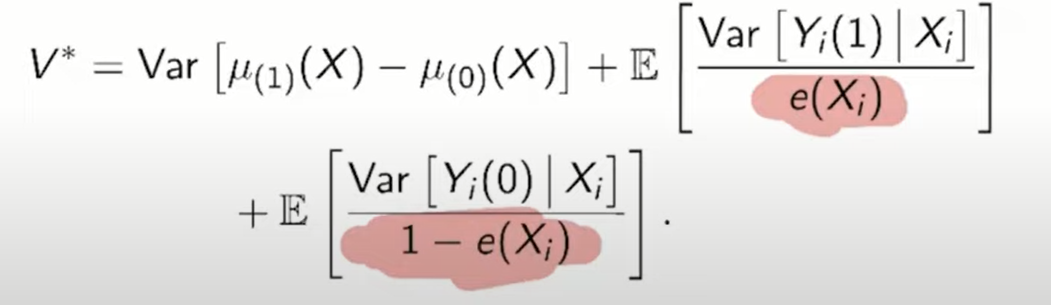
\includegraphics[scale = 0.3]{overlap_variance.png}
    \caption{Overlap on Variance Estimation}
    \label{fig:overlap}
\end{figure}


This is easy to check. Just look if you have a nice histogram and no spikes at 0 and 1. Just do not want clusters ( a lot of observations) around 0 and 1

An example: Athey, Levin, Seira analysis of timer auctions. 

\subsection{Wrapping up ATE estimation}

Treatment effects are imporant in many scientific analyses. Once we have identified treatment effects via unconfoundedness, we can estimate them bu combining flexible machin eleanring methods with augmented IPW
\begin{itemize}
    \item Formally, AIPW yields semi-parametrically efficient estimtes of the treatment effect, provided the inputs from ML methods are accurate enough
    \item In practice, AIPW makes our procedure robust to regularization bias
    \item AIPW allos from simple confidence intervals that do not depend on which specifc ML moethd we used
\end{itemize}

AIPW lets ML focus on what its good at (i.e accurate prediction ), and then uses its outputs for efficient treatment effect estimation.

\begin{figure}[H]
    \centering
    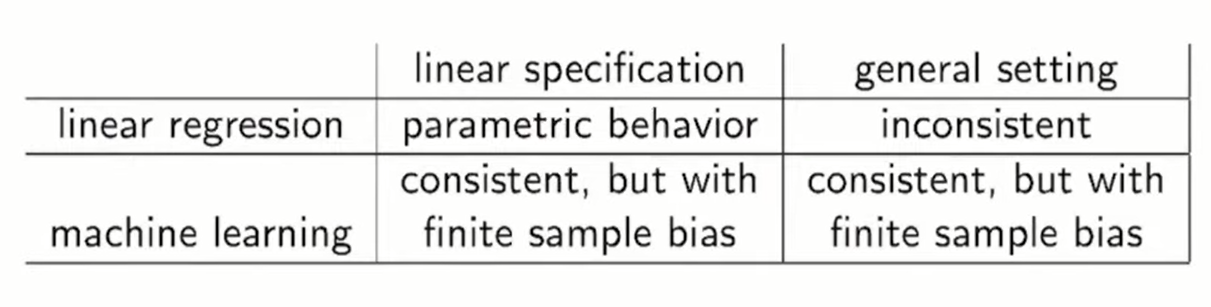
\includegraphics[scale = 0.3]{ml_lm.png}
    \caption{ML and Linear Regression Differences}
    \label{fig:ml_lm}
\end{figure}

ML is consistent but has finite sample bias

When deploying ML in Causal Inference, we need to use strategies that are robust to moderate finite sample errors. In the context of ATE estimate, AIPW is one solution with this property.

Below are some references to check out:


\begin{figure}[H]
    \centering
    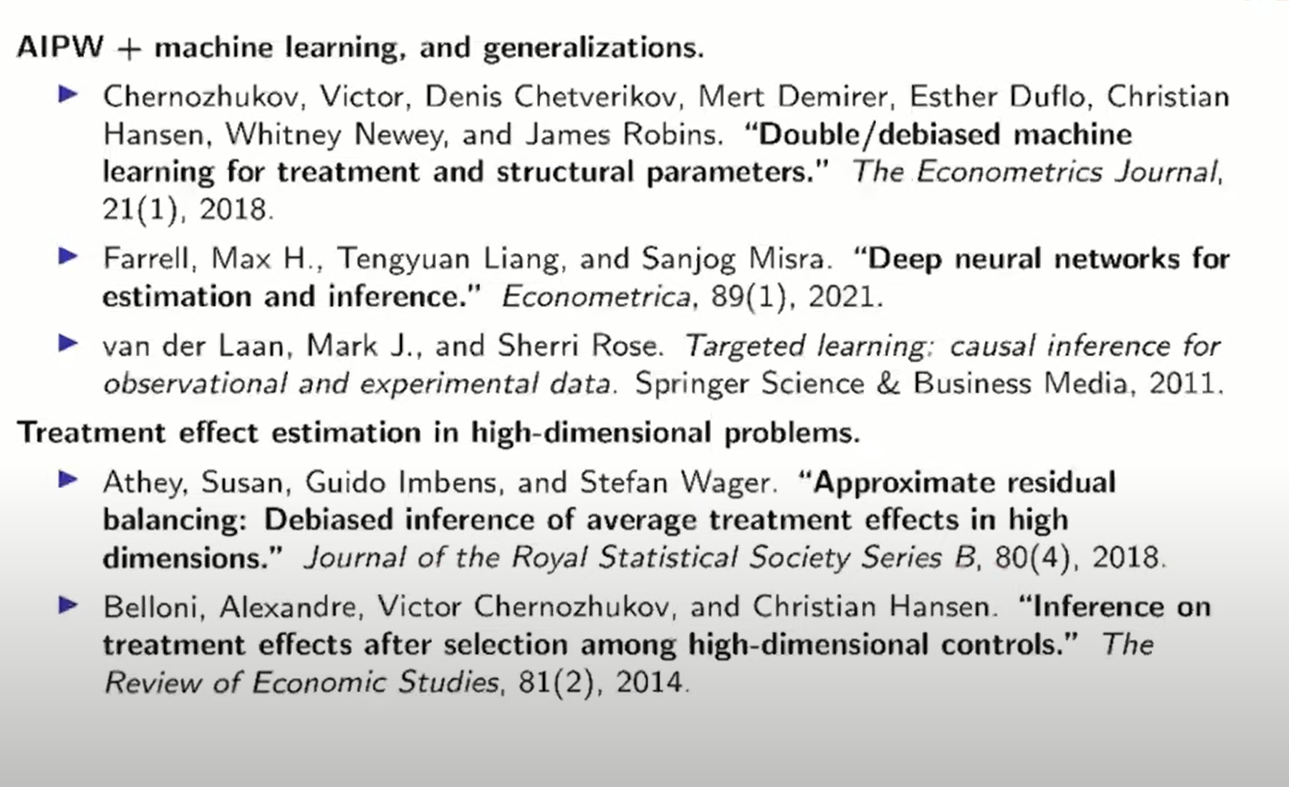
\includegraphics[scale = 0.3]{ref_ate.png}
    \caption{ML ATE References}
    \label{fig:ref}
\end{figure}

\section{Class 9 Conditional Average Treatment Effects: Overview}

Athey "Impact of ML on Economics

Athey \& Imbens "ML methods Economists SHould Know About"

What are ML contributions to Causal Inference?
\begin{itemize}
    \item ATE: Controls for Confounders
    \begin{itemize}
        \item Post-Double Lasso (Belloni, Chenozhukov, and Hansen)
        \item Residual Balancing (Athey, Imbens, and Wagner)
        \item AIPW/Double ML (Chenozhukov et al)
    \end{itemize}
    \item IV
    \begin{itemize}
        \item Slect from many instruments (Chenozhukov et al)
    \end{itemize}
    \item Panel Data
    \begin{itemize}
        \item Matrix factorization as alternative to DID, synthetic controls (Athey)
        \item As part of structural models of consumer behavior (Athey, Blei, Ruiz; Athey at al)
    \end{itemize}
    \item CATE: Heterogeneous treatment effects, optimal policies, adaptive expressiveness
\end{itemize}

How do we find optimal treatment assignment policies? Different individuals/groups respond differently to treamtent. ATE takes the average of this effect whereas CATE breaks the effect up by group. Formally:

\begin{itemize}
    \item Customized to Subpopulations: $E[ \tau | X_i \in S]$
    \item Customized to individual observables: $E[\tau | X_i = x]$
\end{itemize}


Treatment Effect Heterogeneity

\begin{figure}[H]
    \centering
    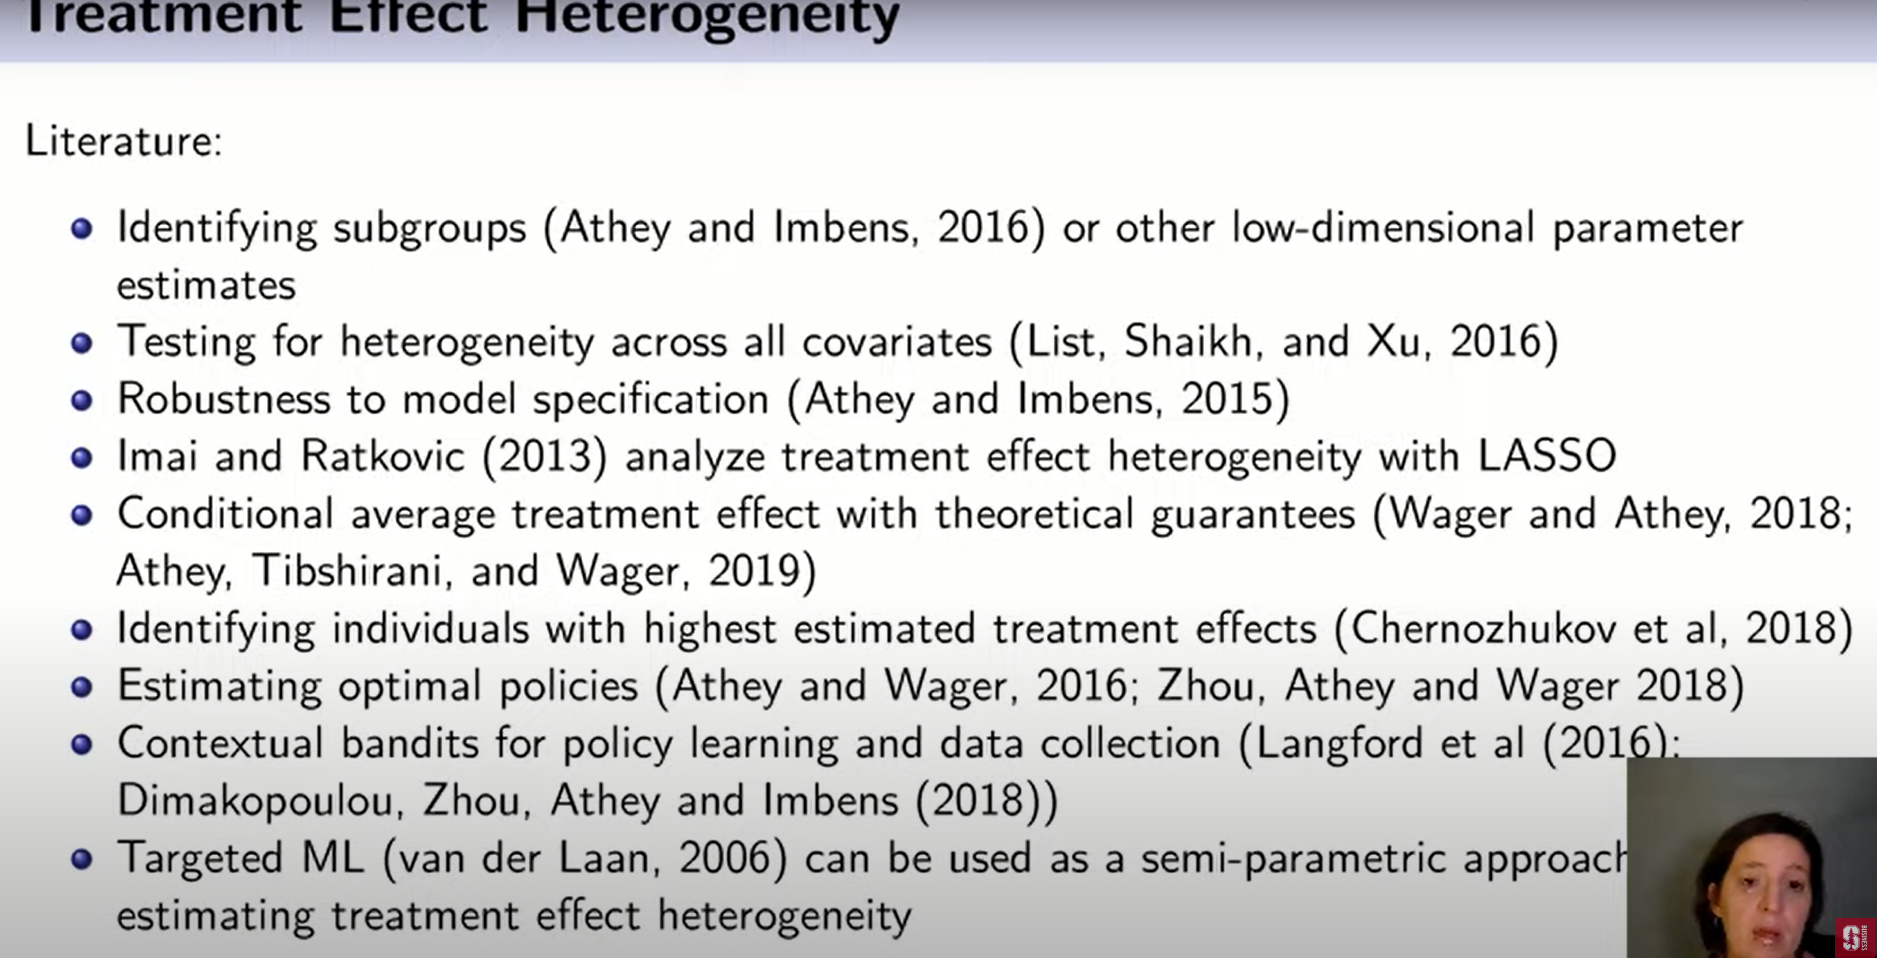
\includegraphics[scale = 0.3]{ref_cate.png}
    \caption{ML CATE References}
    \label{fig:cate_ref}
\end{figure}


ML methods perform well in practice, but many do not have well established statistiacl properties. Unline prediction, ground truth for causal parameters not directly observed. Need valid confidence intervals for many applications (AB testing, drug trials, etc); challenges include adpative model selection and multiple testing

Some themes of ML/CI research agenda:

\begin{itemize}
    \item Either decompose problem into prediction and causal components; or build novel meothds inspired by ML
    \item Sample splitting/cross-fitting to avoid spurios findings and to get consistency/asymptotic normality
    \item build insights from semi-parametric theory
    \item Use orthogonal moments to build in greater tolerance for slow convergence in nuisance parameters.
\end{itemize}




\begin{figure}[H]
    \centering
    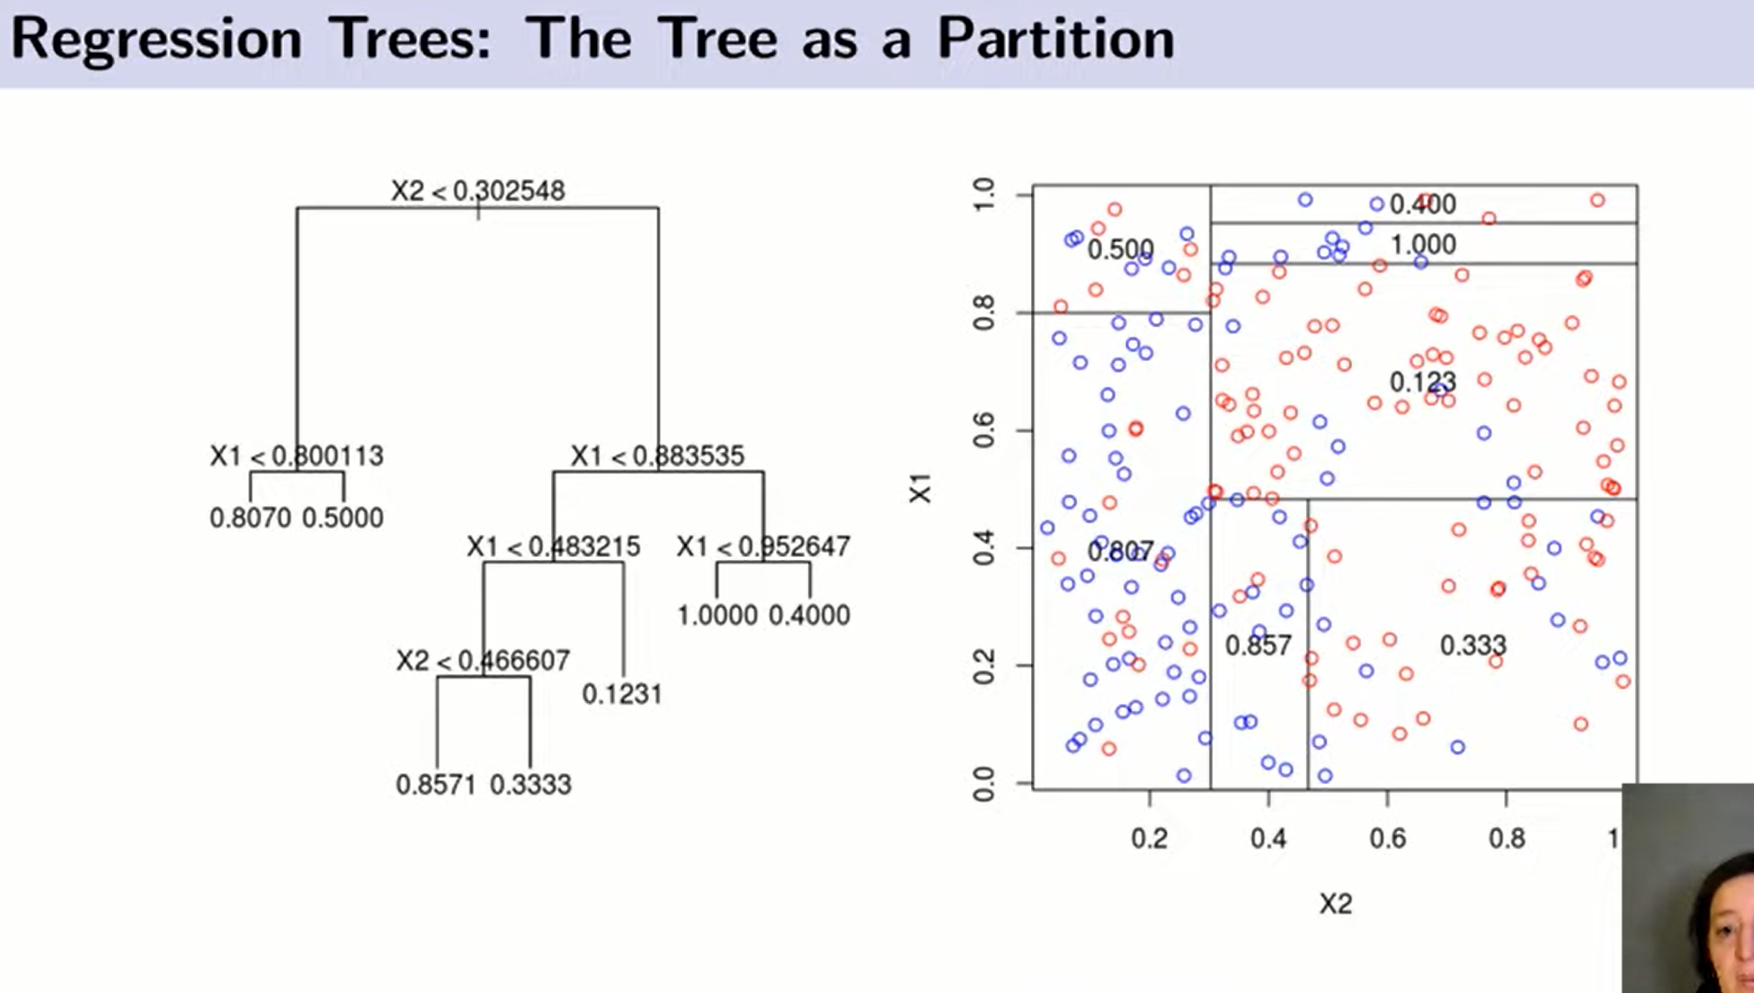
\includegraphics[scale = 0.3]{reg_tree_partition.png}
    \caption{Regression Tree as a Partition}
    \label{fig:reg_partition}
\end{figure}

Causal trees divide popuulation into subgoroups to minimize MSE in treatment effects.
\begin{itemize}
    \item Goal: report heterogeneity without pre-analysis plan but with valid confidence intervals
    \item Moving the goalposts: method defines estimand (treatment effects for subgroups) and generates estimates
    \item Solve for over-fitting problem with sample splitting: choose subgroups in half the sample and estimate on other half
\end{itemize}

\begin{itemize}
    \item Challenges
    \begin{itemize}
        \item object function is infeasible: $\sum_i [(\tau_i - \hat{\tau}(X_i))^2]$
        \item Need to estimate objective to optimize for it rather than take a simple average of squared error
        \item estimand is unstable
    \end{itemize}
\end{itemize}

What are the approaches to getting CATE? see Taxonomy from Athey and Imbens 2016

First, you could build a single model ("single trees): that forces the data to split on treatment effects. If your tree does not split because the machine does not find anything important, then you might have no treatment effect. This is called the "S-Learner"

Second, you could build two separete models for treamtne and control ("two trees"). For a given value x, the neighborhood defined for treatment group might be totally different than control group, e.g. treated tree splits on gender and control tree splits on age. Then male, 60 yrs old, is in the "male" leaf in treatment group treee, and in the "ovre 50" leaf in the control group tree. Estimate of treatment effect heterogeneity compares treated males to older people in control group. This is referred to as the "T-Learner".

Third, you could do the "transformed outcome" method. We could transform the outcome and build a single prediction model that is generalized (e.g Chernozuhov et al) to AIPW score as the outcome.

To transform the outcome you do the following:

Let $p$ be the assignment probability. let $Y^*_i = \frac{Y_i}{p}$ if $W_i=1$, and let $Y^*_i =  - \frac{Y_i}{(1-p)}$ if $W_i = 0$. It is straightforward to check that $E [Y^*_i | X_i = x] = \tau (x)$. It is a noisy, but unbiased estimate of CATE. Thus, if we first transform the outcome, and then apply a prediction method to the transformed outcome, we will get estimates of CATE. This can be generalized in obserational studied to weighting by an estimated propensity score, or use the AIPW score as an outcome.

Fourth, you could estimate the MSE criterion (preferred in Athey and Imbens 2016)


\subsection{Notation for Partitions and Leaf Effect Estimates}

There are three samples that partition according to training and testing $\hat{f}$ on the data $S$:

\begin{itemize}
    \item Model selection / tree construction: $S^{tr}$
    \item Estimation sample for leaf effects $S^{est}$
    \item a (hypothetical) test sample $S^{te}$
\end{itemize}

Partitions are denoted as $\Pi$

$\hat{\tau}(X_i; S^{est}, \Pi)$ is the sample average treatment effect in sample $S^{est}$ for the leaf $l (X_i ; \Pi)$ associated with covariates $X_i$:

\begin{equation}
    \begin{aligned}
        \hat{\tau}(X_i; S^{est}, \Pi) = \frac{1}{\sum_{j \in S^{est} \bigcap l(X_i; \Pi)} W_i } \sum_{j \in S^{est} \bigcap l(X_i; \Pi)} W_i Y_i \\
        - \frac{1}{\sum_{j \in S^{est} \bigcap l(X_i; \Pi)}(1-W_i)}  \sum_{j \in S^{est} \bigcap l(X_i; \Pi)} (1-W_i) Y_i
    \end{aligned}
\end{equation}

Causal Tree Algorithm

\begin{itemize}
    \item Divide data into tree-building $S^{tr}$ and estimation $S^{est}$ samples
    \item Use a greedy algorithm to recursively partition covariate space $\chi$ into a deep partition $\Pi$
    \begin{itemize}
        \item At each node the split is selected as the one that minimise our estimate of EMSE over all possible binary splits
        \item Preserve minimum number of treated and control units in each child leaf
    \end{itemize}
    \item Use cross-validation to select the depth $d^*$ of the partition that minimizes an estimate of MSE of treatment effects, using left-out folds as prxoies for the test set
    \item Select partition $\Pi^*$ by pruning $\Pi$ to depth $d^{*}$, pruning leaves that provide the smallest improvement in goodness of fit
    \item Estimate the treatment effect in each leaf of $\Pi^*$ using the estimation sample $S$ (meant to be $S^{est}$?)
\end{itemize}

\section{Class 10/11 -- CATE: Trees/Forests}

So we have trees that can be made to find CATE. We should have a test-train split on our data to make sure the tree is honest. Let's breakdown the different methods/approaches to trees and forests

\begin{itemize}
    \item Causal Trees
    \begin{itemize}
        \item Move the goalpost so that we are estimating a small number of parameters, but get guaranteed coverage with many observations per parameter and by using sample splitting
        \item Easy to intrepret, easy to mis-interpret
        \item can be many trees
        \item Leaves differ in many was if covariates correlated; describe leaves by means in all covariates
    \end{itemize}
    \item Causal Forests
    \begin{itemize}
        \item Attempt to estimate $\tau(x)$
        \item Can estimate partial effects
        \item In high dimensions, still can have omitted variable issues
        \item Confidence intervals lose coverage in high dimension (bias)
        \item Can be used as an input into estimation of lower dimensional objects, such as average effects for high-CATE individuals or average benefits of a targeted treatment assignment policy
    \end{itemize}
\end{itemize}

Matching in economics is the same as k-NN matching. The k-NN estimator for $\tau(x)$ is:

\begin{equation}
    \hat{\tau} = \frac{1}{k} \sum_{S_1 (x)} Y_i - \frac{1}{k} \sum_{S_0 (x)} Y_i
\end{equation}

This is consistent given unconfoundedness and regularity conditions

\begin{itemize}
    \item \textbf{Pro: } Transparent asymptotics and good, robust performance when p is small
    \item \textbf{Con: } Acute curse of dimensionality, even when p=20 and n=20k
\end{itemize}

k is the number of neighbors.

Random forests are essentially k-NN estimators. Precisely, they a re a heuristic for adaptive nearest neighbors estimations (introduce by Breiman 2001).

\begin{itemize}
    \item \textbf{Pro: } Excellent empirical track record
    \item \textbf{Con: } Often used as a black box without statistical discussion
\end{itemize}

There has been considerable interest in using forest-like methods for treatment effect estiation but without formal theory. Some references of research using forest methods in economics:

\begin{itemize}
    \item \textbf{Bayesian forest algorithms} Green and Kern 2012, Hill 2011, BART Chipman et al 2010
    \item \textbf{Tree based methods } Athey and Imbens 2016, Su et al 2009, Taddy et al 2014, Wang and Rudin 2015, Zeilis et al 2008 
    \item \textbf{Asymptotic inference} Wager and Athey 2018 provide the first formal results allowing random forest to be used for provably valid asymptotic inference
\end{itemize}

What is a causal tree? Athey and Imbens (2016) introduce the causal treee: defines neighborhoods for matching based on recursive partitioning (Breiman, Friendman, Olshen, Stone 1984), advocate sample splitting (w/ modified splitting rule) to get assumption-free confidence intervals for treatment effects in each leaf.

How to go from trees to forests? Suppose we have a training set ${(X_i,Y_i,W_i)^n _{i=1}}$, a test point $x$, and a tree predictor:

\begin{equation}
    \hat{\tau(x)} = T(x ; {(X_i,Y_i,W_i)^n _{i=1}})
\end{equation}

Random forest idea: build and average many different trees:


\begin{equation}
    \hat{\tau(x)} = \frac{1}{B} \sum_{b=1}^B  T^* _b(x ; {(X_i,Y_i,W_i)^n _{i=1}})
\end{equation}

Where $B$ is the total number of trees $b$ created.

We turn $T$ into $T^*$ by: 
\begin{itemize}
    \item Bagging / sub-sampling the training set (Breiman, 1996); this helps smooth over discontinuities (Buhlmann and Yu, 2002)
    \item Selecting the splitting variable at each step from $m$ out of $p$ randomly drawn features (dimensions) (Amit and Geman, 1997)
\end{itemize}

Because Honest trees do not use the same data to select partition (splits) and make predictions (Wager and Athey 2018) we need to a forest to smooth over. Regression forests are asymptotically Gaussian and centered given the following assumptions:

\begin{itemize}
    \item Honesty: individual trees are honest
    \item Sub-sampling: Individual trees built on random sub-samples of size $s  n^\beta$, where $\beta_{min} < \beta < 1$
    \item Continuous features: Features, $X_i$, have a density that is bounded away from 0 and $\infty$ 
    \item Lipschitz response: Conditional mean function $\mu (x) - E [Y | X = x]$ is Lipschitz continuous.
\end{itemize}

Applications in Economics and Marketing:
\begin{itemize}
    \item Hitsch and Misra (2017): causal forests to target catalog mailings. Casaul forest detects significant heterogeneity, performs better than alternative including LASSO and off-the-shelf random forest
    \item Davis and Hell (2017): Analyze heterogeneous impacts of summer jobs using causal forest
    \item Athey, Kelleher, and Spiess (2021): Applications for financial aid
\end{itemize}

\subsection{Robustness of CATE}

How do we know we really have CATE instead of ATE? When estimating, common in prediction models to assess calibration. One approach is to estimate trhe slope of the relationship between actual and predited CATE. Slope of 1 is well calibrated; slope above zero is evidence of heterogeneity. This comes from Chenozhukov, Demier, Duflo, Fernandez-Val, 2018. This is how we can test and quantify heterogeneity.

Another way that we can quantify heterogeneity is by comparing ATE by quantiles of sorted CATE. Here we can hold out fold $k$ of the data. On the remaining data estimate CATE and define a mapping $\hat{Q}_{-k}$ from $x$ to , e.g, quartiles of the CATE distribution. Apply $Q_{-k}$ to the covariate values $x$ in fold $k$. Repeat this for all folds; at that point, each observation has been assigned to one of the four quartiles. Finally, estimate the ATE by quartile.

Lastly, another way to test for heterogeneity is to compare the means and standard errors at each end of the CATE distribution. You can split by all covariates and compare deciles 1 and 10. If statistically different from each other, then you have HTE or CATE.

\subsection{Forest Weakness}

When are forests the weakest? 
\begin{itemize}
    \item Many economic datasets have smooth relationships
    \item Many relationships are monotonic or U-shaped
    \item Forests fit a line as a step function
    \item A variety of ML methods might improve but little theory
    \item \textbf{Solution: Local Linear Forests + Theory}
\end{itemize}

Local Linear forests have very good properties (can fit to data on the extremes better than CF). see Friedberg, Athey, Tibshirani and Wager 2018


\section{Class 13: Heterogeneous Treatment Effects: Sources of Bias}

\subsection{The Partially Linear Model}

For future reference: under constant treatment effects where each individual has the same treatment effect (different from ATE where $ATE = E [\tau (X)]$ for a potentially hetergenous function $\tau (.)$, we have a semi-parametric problem. Given that we get a partially linear model out of assuming constant treatment effects:

\begin{equation}
    E [ Y | X =x, W =x] = \mu_{(0)} (x) + w \tau
\end{equation}

There exist a low-dimensional parameter of interest $\tau$ but have a non-parametric nuisance component \footnote{nuisance just means that we need to estimate but are not interested in its efects`} $\mu_{(0)} (x)$. This means that we have a coefficient we want to estimate and a bunch of confounders we want to isolate their effects away (make exogenous to) from our treatment effect. Robinson (1988) proposed a simple approach to estimation in this model, based on the following observation. Defining 

\begin{equation}
\begin{aligned}
    e (x) = E [W_i | X_i = x], and \\
    m (x) = E [Y_i | X_i = x] = \mu_{(0)} (x) and \tau e(x),
\end{aligned}
\end{equation}

we can re-write the partially linear model as 

\begin{equation}
    Y_i - m(X_i) = \tau (W_i - e (X_i)) + \epsilon_i , E [\epsilon_i | X_i , W_i] = 0
\end{equation}

How do we run this model: it follows a three step approach

\begin{enumerate}
    \item Get an estimate $\hat{e}(.)$ (estimated residuals) by predicting $W_i$ from $X_i$
    \item Get an estimate $\hat{m}(.)$ by predicting $Y_i$ from $X_i$
    \item Estimate $\tau$ by \textbf{residual-on-residual regression}
\end{enumerate}

\begin{equation}
    \hat{\tau} = \sum_{i=1}^n (Y_i - \hat{m} (X_i)) (W_i - \hat{e}(X_i)) / \sum_{i=1}^n (W_i - \hat{e}(X_i))^2
\end{equation}

Doing this with OLS:

\begin{enumerate}
    \item Fit linear model $W_i \sim X_i \gamma_e$
    \item Fit a linear model $Y_i \sim X_i \gamma_m$
    \item Same as equation above but replace $\hat{m}(.)$ and $\hat{e}(.)$ with $X_i \hat{\gamma}_e$ and $X_i \hat{\gamma}_m$, respectively
\end{enumerate}


We've now gone over two "robust" estimators in this class:

\begin{itemize}
    \item The AIPW estimator for the ATE
    \item The residual-on-residual regression for a constant treatment effect
\end{itemize}

Both estimators have the propertry that if "nusiance components" (i.e non-focal parts of the problem") are estimated reasonably accurately, then we get $1 / \sqrt{n}$ rate central limit theorom for our target estimand. These are two special cases of a general recipe for robust, semi-paramentric causal inference. For more see Chernozhukov Escanciano Ichinmura Newey Robins 2016

To reiterate: Estimating constant treatment effect $\tau (X) = \tau$ is not the same problem as estimating an average treatment effect i.e $ATE = E [ \tau (X)]$ for a potentiall heterogeneous function $\tau(.)$
\begin{itemize}
    \item To estimate an \textbf{average effect} we need reasonably accurate estimates of $\tau (x)$ everywhere
    \item To estimate a constant effect we can opportunistically focus on areas with the most signal
\end{itemize}



\begin{figure}[H]
    \centering
    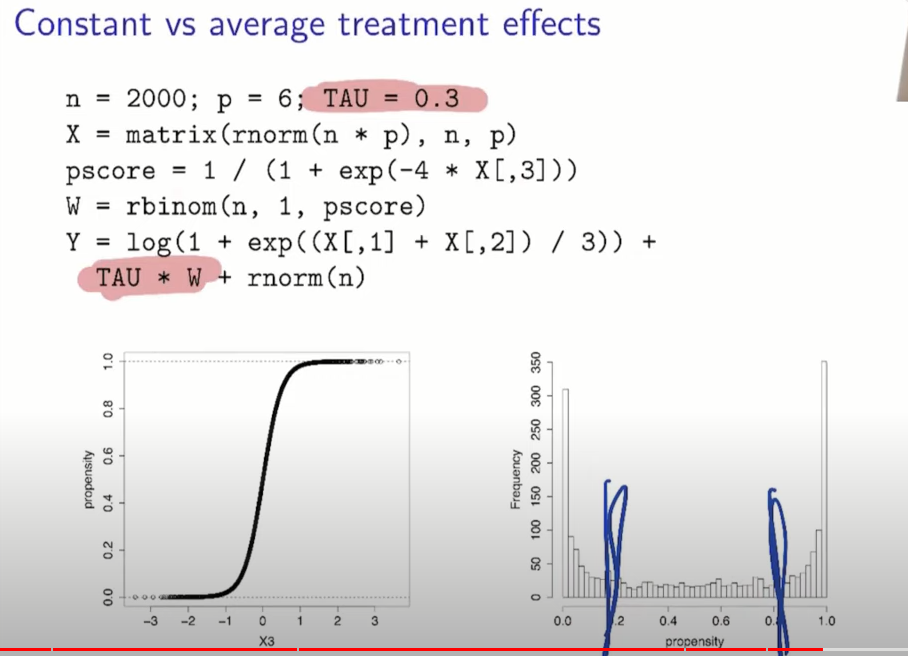
\includegraphics[scale = 0.3]{r_code.png}
    \caption{R code for simulation}
    \label{fig:reg_partition}
\end{figure}




\end{document}

